%\section{Anytime Control Robust MPC}

In this paper, we design the controller using a Robust Model Predictive
Control (RMPC) approach via constraint restriction \cite{richardsetal05rmp, chiscietal01swp}.
In order to ensure robust safety and feasibility, the key idea of
this approach is to tighten the state constraint iteratively to account
for possible effect of the disturbances. As time progresses, this ``robustness
margin'' is used in the MPC optimization with the nominal dynamics,
\ie the original dynamics where the disturbances are either removed
or replaced by nominal disturbances.
%An advantage of this approach is that, 
Because only the nominal dynamics are used, the complexity of the optimization is the same as for the nominal problem.

\begin{comment}
Since the controller only has access to the state estimate $\hat{x}_{k}$
but not the plant's state $x_{k}$, conceptually the control system
structure is arranged as in \figref{conceptual-system-diagram}.
From the controller's point of view, the\emph{ plant }that it controls consists of both the physical plant, whose state is hidden, and the
estimator, whose state is exposed to the controller. This composed
plant is called a \emph{virtual plant}. Although the exact state $x_{k}$
is hidden from the controller, it is within an unknown but bounded
distance from the state estimate. With this knowledge, the controller
can compute the control input so that robust safety and feasibility
are achieved, and it can also adjust the estimation accuracy appropriately.

\begin{figure}
\centering{}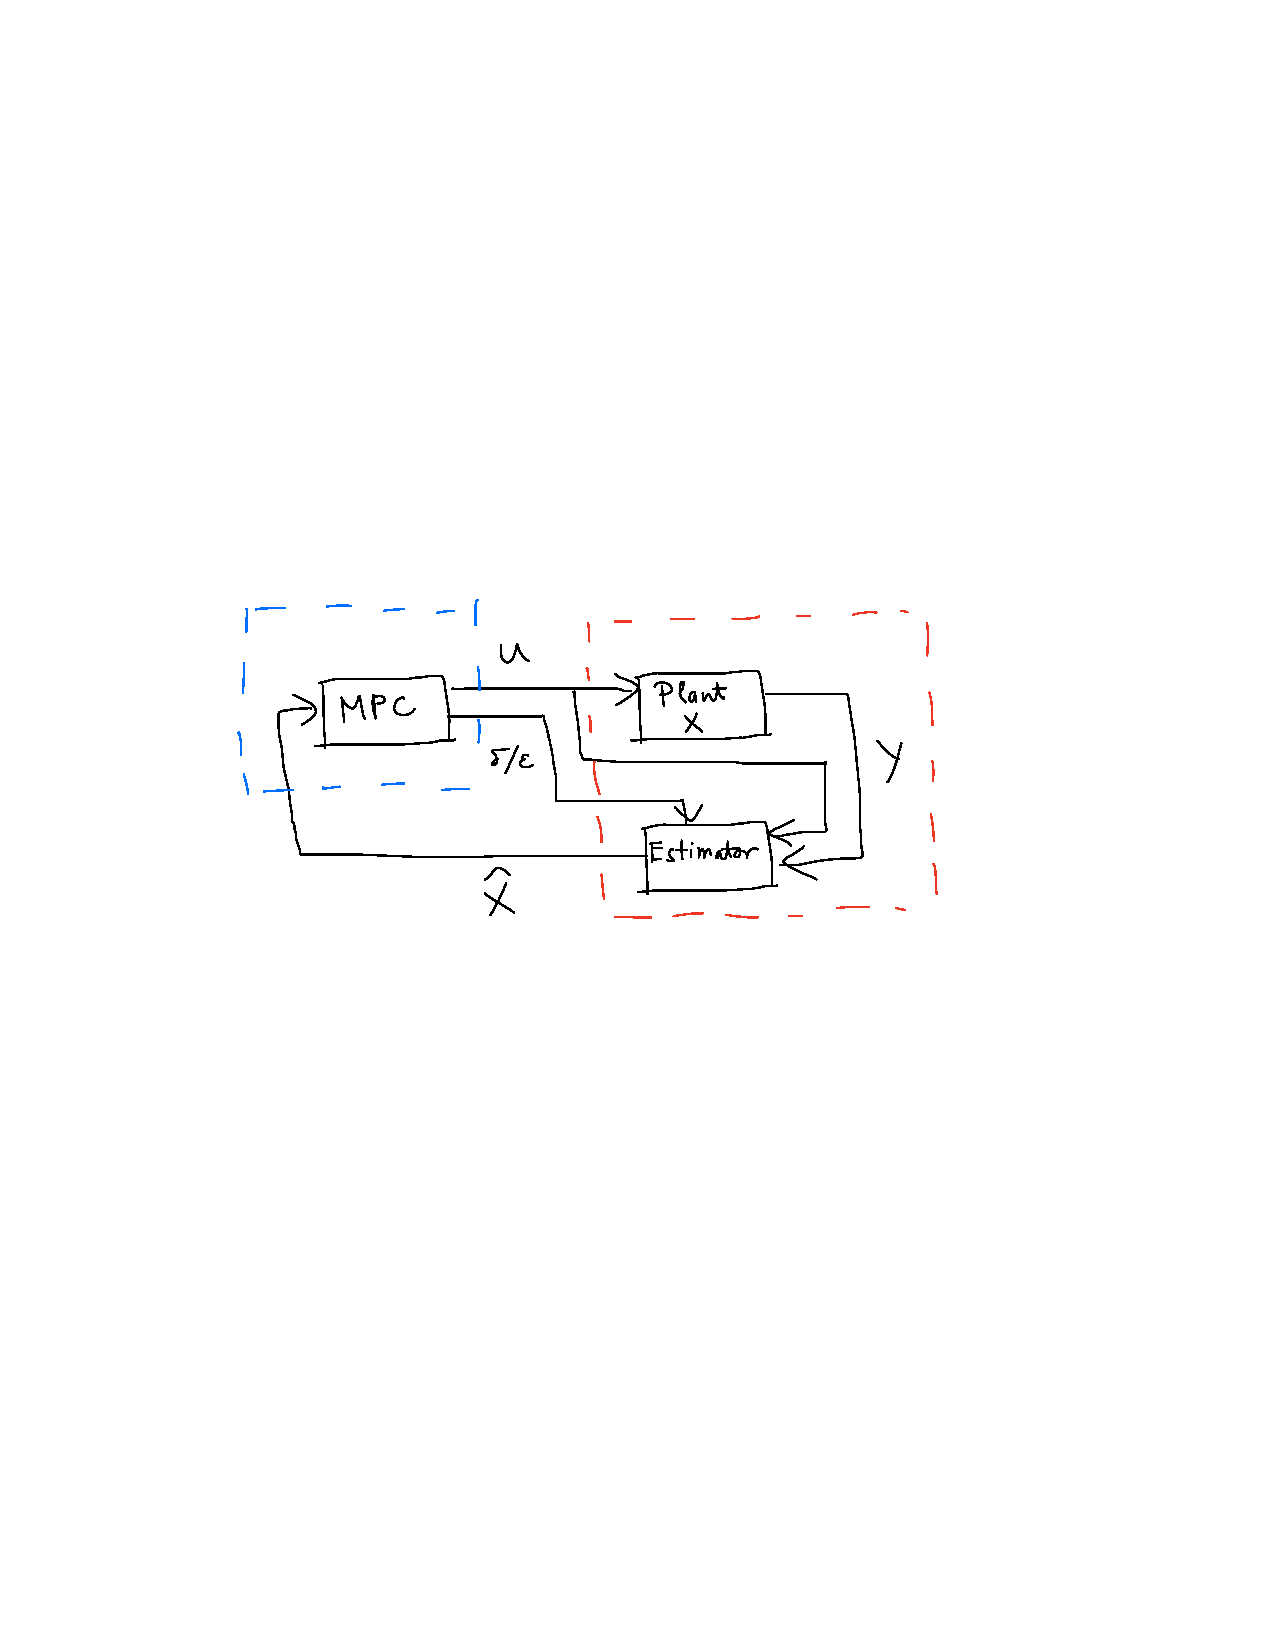
\includegraphics{figs/conceptual_system}\caption{Conceptual structural diagram of the control system for control design.}
\label{fig:conceptual-system-diagram}
\end{figure}
\end{comment}


Since the controller only has access to the estimated state $\hat{x}$, we need
to rewrite the plant's dynamics with respect to $\hat{x}$. The error
between $ $$x_{k}$ and $\hat{x}_{k}$ is $e_{k}=x_{k}-\hat{x}_{k}$.
At time step $k+1$ we have
\begin{align*}
\hat{x}_{k+1} & =x_{k+1}-e_{k+1}\\
 & =Ax_{k}+B_{1}(\sDelay[k])u_{k-1}+B_{2}(\sDelay[k])u_{k}+w_{k}-e_{k+1}\text{,}
\end{align*}
 then, by writing $x_{k}=\hat{x}_{k}+e_{k}$, we obtain the dynamics
\begin{equation}
\hat{x}_{k+1}=A\hat{x}_{k}+B_{1}(\sDelay[k])u_{k-1}+B_{2}(\sDelay[k])u_{k}+\hat{w}_{k},\quad k\geq0\label{eq:estimator-dynamics}
\end{equation}
 where $\hat{w}_{k}=w_{k}+Ae_{k}-e_{k+1}$.
The set of possible values of $\hat{w}_{k}$
depends on the estimation accuracy at steps $k$ and $k+1$ and is
denoted by $\WhSet(\sAccu[k],\sAccu[k+1])$, \ie
$\WhSet(\sAccu,\sAccu')\definedas\left\{ w+Ae-e'\SuchThat w\in\WSet,e\in\ESet(\sAccu),e'\in\ESet(\sAccu')\right\}$.
Note that %we assume
$\WhSet(\sAccu[k],\sAccu[k+1])$ is independent
of the time step $k$. %
It can be computed as $\WhSet(\sAccu,\sAccu')=\WSet\oplus A\ESet(\sAccu)\oplus\left(-\ESet(\sAccu')\right)$
where the symbol $\oplus$ denotes the Minkowski sum of two sets.

%\shadowbox{\begin{minipage}[t]{1\columnwidth}%
%Truong: It's important to note here that I used $e_{k}=x_{k}-\hat{x}_{k}$,
%so the implementation code should be double checked to match this
%definition.%
%\end{minipage}}

The dynamics in \eqref{estimator-dynamics} has a nonstandard form
where it depends on both the current and the previous control inputs.
However we can expand the state variable to store the previous control
input as
\[
\hat{z}_{k}=\begin{bmatrix}\hat{x}_{k}\\
u_{k-1}
\end{bmatrix}\in\RR^{n+m}
\]
and rewrite the dynamics as, for all $k\geq0$,
\begin{equation}
\hat{z}_{k+1}=\hat{A}(\sDelay[k])\hat{z}_{k}+\hat{B}(\sDelay[k])u_{k}+\hat{F}\hat{w}_{k}\text{.}\label{eq:estimator-std-dynamics}
\end{equation}
Here, the system matrices are
\begin{equation}
\begin{gathered}
\hat{A}(\sDelay[k])=\begin{bmatrix}A & B_{1}(\sDelay[k])\\
\bm{0}_{m\times n} & \bm{0}_{m\times m}
\end{bmatrix},\\
\hat{B}(\sDelay[k])=\begin{bmatrix}B_{2}(\sDelay[k])\\
\IdentityMatrix_{m}
\end{bmatrix},\quad\hat{F}=\begin{bmatrix}\IdentityMatrix_{n}\\
\bm{0}_{m\times n}
\end{bmatrix}\text{.}
\end{gathered}
\label{eq:lifted-matrices}
\end{equation}

Let the actual expanded state be $z_{k}=\left[x_{k}^{T},u_{k-1}^{T}\right]^{T}$.
Because the expanded state consists of both the plant's state and
the previous control input, the state constraint $x_{k}\in\XSet$
and the control constraint $u_{k}\in\USet$ are equivalent to the
joint constraint $z_{k}\in\XSet\times\USet$. We can now describe
the RMPC algorithm for the dynamics in \eqref{estimator-std-dynamics}.


\subsection{Tractable RMPC Algorithm}

Let $N\geq1$ %
\begin{comment}
May need to change the smallest N
\end{comment}
{} be the horizon length of the RMPC optimization. Because the system
matrices in the state equation~(\ref{eq:estimator-std-dynamics})
depend nonlinearly on the variables $\sDelay[k]$, the RMPC optimization
is generally a mixed-integer nonlinear program, which is very hard
to solve. To simplify the RMPC optimization to make it tractable, we fix the estimation mode for the entire RMPC horizon.

Let $\MPCProb{\sDelay,\sAccu}(\hat{x}_{k},\sDelay[k],\sAccu[k],u_{k-1})$
denote the RMPC optimization problem at step $k\geq0$ where the current
state estimate is $\hat{x}_{k}$, the current estimation mode is $(\sDelay[k],\sAccu[k])\in\Delta$,
the previous control input is $u_{k-1}$, and the estimation mode
for the entire horizon (after step $k$) is fixed at $(\sDelay,\sAccu)\in\Delta$.
The specific RMPC optimization formulation will be presented in \secref{RMPC-Formulation}.
Because the estimation mode is fixed for the RMPC optimization, the
RMPC cost function only needs to include the first component of $J$:
$J_{\sDelay,\sAccu}=\sum_{j=k}^{k+N}\ell(x_{j},u_{j})$. The estimation
and computation cost will be added later $J_{\sDelay,\sAccu}^{\mathrm{total}}=J_{\sDelay,\sAccu}^{\star}+\alpha\pi(\sDelay)$
where $\alpha\geq0$ is a %positive
weight specified by the designer.
Since the system matrices become constant now, if the stage cost $\ell(\cdot)$
is linear or positive semidefinite quadratic, each optimization problem
$\MPCProb{\sDelay,\sAccu}(\cdot)$ is tractable and can be solved
efficiently as we will show later. The RMPC algorithm with Anytime Estimation is stated in \algoref{RMPC-algo}.

\begin{algorithm}
\begin{algorithmic}[1]
\State $\left(\sDelay[0], \sAccu[0]\right)$ and $u_{-1}$ specified by designer
\State Apply $u_{-1}$
\For{$k=0,1,\dots$}
	\State Estimate $\hat{x}_{k}$ with mode $\left(\sDelay[k], \sAccu[k]\right)$
	\For{each $\left( \sDelay,\sAccu \right) \in \Delta$}
		\State Solve $\MPCProb{\sDelay,\sAccu}(\hat{x}_{k},\sDelay[k],\sAccu[k],u_{k-1})$
		\State Calculate cost $J_{\sDelay,\sAccu}^{\mathrm{total}} = J_{\sDelay,\sAccu}^{\star} + \alpha \pi(\sDelay)$
	\EndFor
	\State $( \sDelay^{\star}, \sAccu^{\star}, u_{k \Given k}^{\star} ) \gets \argmin_{\sDelay,\sAccu} J_{\sDelay,\sAccu}^{\mathrm{total}}$
	\State Wait until $t_{a,k}$
	\State Apply control input $u_{k} = u_{k \Given k}^{\star}$ and estimation mode $\left( \sDelay[k+1], \sAccu[k+1] \right) = \left( \sDelay^{\star}, \sAccu^{\star} \right)$
\EndFor
\end{algorithmic} 

\caption{RMPC algorithm with Anytime Estimation.}
\label{algo:RMPC-algo}
\end{algorithm}

%%% Local Variables: 
%%% mode: latex
%%% TeX-master: "CDC14_Anytime_Main"
%%% End: 
